\section{Career Path Results}
\label{sect:career-path-results}
Examples of the JSON objects returned by the career mapping portion of the
ProGENitor code are shown below.  Each example does not contain a complete set
of data as that would be too much to show in this report.

\subsection{Node Interconnect JSON Results}
In the node interconnect JSON Object, an array of node interconnections is
returned.  Each element of the array contains a starting node and an ending node
for the transition.  Additionally, the array element also contains a transition
frequency.  The transition frequency indicates how often the transition occurs. 
Currently this is on a scale of 0-10, so that user data is not exposed to the
ProGENitor users.  Thus, the actual number of users transitioning from one node
to another node is divided by the total number of users that data was pulled for
the career map.  This percentage is then multiplied by 10 and rounded.

\noindent\{"Node Connections":\\*
\{"node A":"Bachelors","node B":"Masters","transition frequency":6\},\\*
\{"node A":"Masters","node 	B":"Circuit Designer","transition frequency":7\},\\*
\{"node A":"Circuit Designer","node B":"Block 	Owner","transition
frequency":8\},\\* \{"node A":"Block Owner","node B":"Design Owner","transition
frequency":9\},\\*
\ldots\\* 
\{"node A":"Coder","node B":"Function Lead","transition frequency":0\},\\*
\{"node A":"Function Lead","node B":"Masters","transition frequency":0\}]\},\\*


\subsection{Node Ordering JSON Results}
In the node ordering JSON Object, an array containing the order which the nodes
should be display is returned.  Each element of the array contains a node name
and the order number it should be displayed.  Thus, the nodes with an order of
1 should be the first nodes displayed in the career path map, then
moving sequentially up, each node in the group should be displayed until the
final node group is displayed.  This will allow the map to flow with minimum
interconnects flowing in the reverse order.

\noindent \{"Node Ordering":\\*
	\indent\{"node	name":"Timing","order":"2"\},\\*
	\indent\{"node name":"Signal Integrity","order":"2"\},\\*
	\indent\{"node name":"Platform Chief Engineer","order":"7"\},\\*
	\indent\{"node name":"PHD","order":"5"\},\\*
	\indent\{"node name":"Entry Coder","order":"1"\},\\*
	\indent\ldots\\*
	\indent\{"node name":"Block Owner","order":"6"\},\\*
	\indent\{"node name":"Chiplet Designer","order":"1"\}]\},\\*


\subsection{Node Details JSON Results}
In the node detail JSON Object, an Array containing all of the various nodes
will be returned.  Each node will be nested object containing an array of data
points.  Examples of these data points are titles, companies, time spent at the
node, and any other points of interest within the database.  Each of these data
points will be an Object that also contains a nested JSON array.  This array
will then contain data about each data point, broken down into the percentage of
users who matched a specific piece of information for that data point.  For
example, shown below is a data point for the companies that users worked for
when they worked at a Timing job.  To protect user data, this is not shown as
number of users, but as the percentage of users who spent time working for one
company versus all users who spent time working at that particular job.  To
avoid having millions of entries, a threshold is set such that if the threshold
is not met, the data is lumped into an Other group.  This Other group would then
contain the total user data that did not meet the threshold.  Finally, a JSON
Object containing any significant data points is also returned.  ProGENitor
compares the users who reached the goal against all users who passed through the
node to determine what was statistically different from the users who reached
the target goal.  These differences are listed in the significant data object.

\noindent \{"Nodes Data":\\*
	\indent \{"Node Name":"Timing","Node Data":\\*
		\indent \{"Data Breakout":\\*
		\indent \indent	\{"name":"Other","value":"0.9174312\%"\}\\*
		\indent	\indent \{"name":"Timing\_all","value":"100.0\%"\},\\*
		\indent	"Data Point Name":"title"\},\\*
		\indent\{"Data Breakout":\\*
		\indent	\indent	\{"name":"Verizon","value":"100.0\%"\},\\*
		\indent	\indent	\{"name":"Verizon\_all","value":"11.33721\%"\},\\*
		\indent	\indent	\{"name":"Cisco Systems\_all","value":"12.790698\%"\},\\*
		\indent	\indent	\{"name":"Boeing\_all","value":"7.5581393\%"\},\\*
		\indent	\indent	\{"name":"Hewlit-Packard\_all","value":"8.139535\%"\},\\*
		\indent	\indent	\{"name":"IBM\_all","value":"7.2674417\%"\},\\*
		
		\indent	\indent	\{"name":"General Motors\_all","value":"8.72093\%"\},\\*
		\indent	\indent	\{"name":"General Electric\_all","value":"7.2674417\%"\},\\*
		\indent	\indent	\{"name":"Microsoft\_all","value":"8.72093\%"\},\\*
		\indent	\indent	\{"name":"Intel\_all","value":"8.72093\%"\},\\*
		\indent	\indent	\{"name":"Lockheed Martin\_all","value":"11.046512\%"\},\\*
		\indent	\indent	\{"name":"AT\&T\_all","value":"8.430233\%"\},\\*
		\indent"Data Point Name":"company"\},\\*
		\indent\ldots\\*
		\indent \{"Significant":\}\},\\*

\subsection{Example Carrer Map 1}
With the ProGENitor tool, several examples of functionality can easily be
demonstrated.  First, looking at a user that is interested in what it takes to
become a partner in an architecture firm.  The user would submit the query on
Partner and the career map shown in figure \ref{fig:partner nodal map} would be
returned.

\usetikzlibrary{shapes,arrows,chains}

\begin{figure}[H]
	\centering
  
% Start the picture
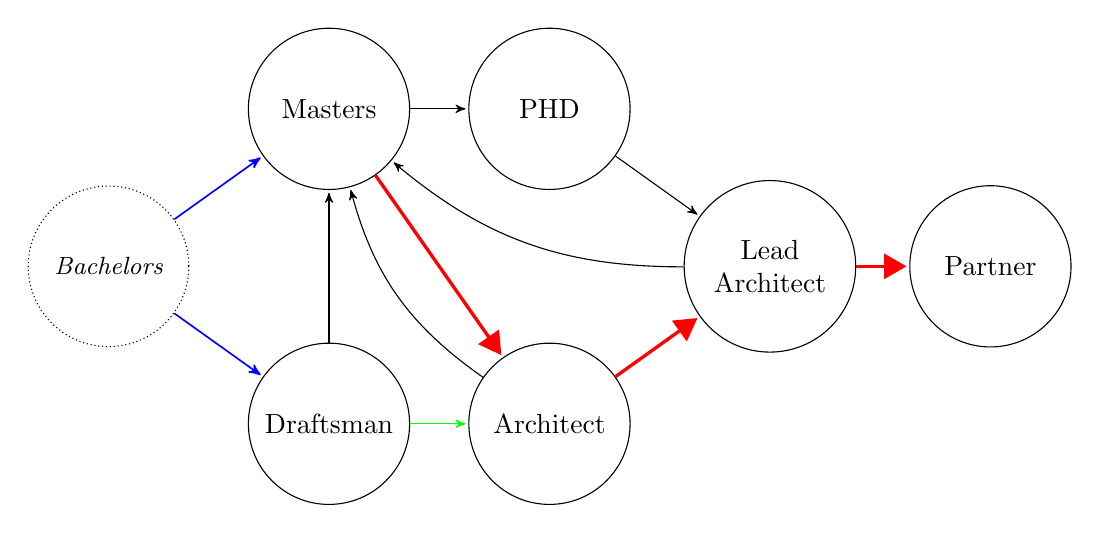
\begin{tikzpicture}[%
    >=triangle 60,              % Nice arrows; your taste may be different
    start chain=going below,    % General flow is top-to-bottom
    node distance=3mm and 28mm, % Global setup of box spacing
    every join/.style={norm},   % Default linetype for connecting boxes
    ]
% ------------------------------------------------- 
% A few box styles 
% <on chain> *and* <on grid> reduce the need for manual relative
% positioning of nodes
\tikzset{
  base/.style={draw, on chain, on grid, align=center, minimum height=2ex},
  node/.style={base, circle, text width=5em},
  % Connector line styles for different parts of the diagram
  norm/.style={->, draw},
  thin/.style={->,>=stealth',shorten >=1pt, black},
  nm/.style={->,>=stealth',shorten >=1pt, green},
  to/.style={->,>=stealth',shorten >=1pt,semithick,blue},
  thick/.style={->,shorten >=1pt,very thick, red},
  it/.style={font={\small\itshape}}
}
% -------------------------------------------------
% Start by placing the nodes
\node [node, densely dotted, it] (a) {Bachelors};
% Use join to connect a node to the previous one 
\node [node, right = of a, yshift=20mm] (b) {Masters};
\node [node, right = of a, yshift=-20mm] (c) {Draftsman}; 
\node [node, right = of b](d) {PHD};
\node [node, right = of c](e) {Architect};
\node [node, right = of e, yshift=20mm](f) {Lead Architect};
\node [node, right = of f](g) {Partner};

\draw [to] (a) to (c);%Bachelors,Draftsman,4
\draw [thin] (c) to (b);	%Draftsman,Masters,1
\draw[thick] (b) to (e);	%Masters,Architect,7
\draw[thick] (e) to (f);	%Architect,Lead Architect,7
\draw[thick] (f) to (g);	%Lead Architect,Partner,7
\draw[to] (a) to (b);	%Bachelors,Masters,5
\draw[thin] (b) to (d); %Masters,PHD,0
\draw[thin] (d) to (f);	%PHD,Lead Architect,0
\draw[nm] (c) to (e);	%Draftsman,Architect,2
\draw[thin] (e) to [bend left=20] (b);	%Architect,Masters,0
\draw[thin] (f) to [bend left=20] (b);	%Lead
% Architect,Masters,0

% -------------------------------------------------
\end{tikzpicture}

	\caption{Career Path Nodal Map}
	\label{fig:partner nodal map}
\end{figure}

This map quickly shows the user that a Bachelors degree is required.  Next the
users can see that a Master's degree could help them move into an architect
role right away versus starting out as a Draftsman.  In either case, both
options can eventually lead to the desired Partner position, with no major
indicator which one yielded a higher likelihood of achieving the goal.  It also
shows that it is rare for someone to return for a Master's degree once they've
entered the workforce and doing so later in your career can actually set the
users back, if they've moved up to a Lead Architect position.  Finally, very
few people who reached the Partner status also obtained a PHD, showing that this
is not a necessary step to achieve this goal.

For additional information, the user could then select one of the nodes to pull
up information about that node.  The three pie charts below in figure
\ref{fig:Lead Arch} show the information that would be returned if the user
were to select the Lead Architect node.  These charts show that there were five
key employers for all of the users who reached Partner.  They also show that
most of the Partners were Lead Architects for less than five years, and it
became increasingly rare to reach Partner after this time.  The data also shows
that no particular city had Lead Architects getting promoted to Partner more
frequently.  Thus, any Lead Architects looking at this data would know to reach
Partner they need to be focused on doing so within the five year window or they
can expect their chances of doing so to diminish over time.  Also, they should
know that where and who they work for is not important as long as they work for
one of the five companies shown.

Alternatively, the user could click on the Master's degree node, to see more
information about these users.  In doing so, the data in generated immediately
shows everyone got a Master's degree in Infrastructure and did so in a single
year.  The only variation is in the school attended.  In this case there were
eight different schools attended, but none was attended at a more significant
frequency than the rest.  Thus the user could immediately know if they wished to
reach partner and do so by obtaining their Master's degree they need to do so by
attending one of these eight schools and get an Infrastructure degree within a
year.


\begin{figure}[H]
\centering

\hspace*{-3cm}\begin{subfigure}[h]{.5\textwidth}
	\centering
	% Pie chart with colors
	% Author: Henri Menke
	\def\angle{0}
	\def\radius{3}
	\def\cyclelist{{"orange","blue","red","green"}}
	\newcount\cyclecount \cyclecount=-1
	\newcount\ind \ind=-1
	\resizebox {88mm} {!} {
	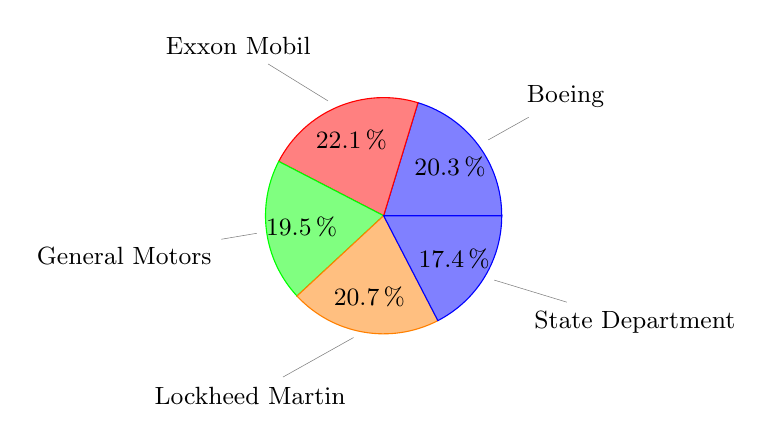
\begin{tikzpicture}[nodes = {font=\small},scale=.5]
  		\foreach \percent/\name in {
      		20.3/Boeing,
      		22.1/Exxon Mobil,
      		19.5/General Motors,
      		20.7/Lockheed Martin,
      		17.4/State Department
    	} {
      		\ifx\percent\empty\else               % If \percent is empty, do nothing
        	\global\advance\cyclecount by 1     % Advance cyclecount
        	\global\advance\ind by 1            % Advance list index
        	\ifnum3<\cyclecount                 % If cyclecount is larger than list
          	\global\cyclecount=0              %   reset cyclecount and
          	\global\ind=0                     %   reset list index
        	\fi
        	\pgfmathparse{\cyclelist[\the\ind]} % Get color from cycle list
        	\edef\color{\pgfmathresult}         %   and store as \color
        	% Draw angle and set labels
        	\draw[fill={\color!50},draw={\color}] (0,0) -- (\angle:\radius)
          		arc (\angle:\angle+\percent*3.6:\radius) -- cycle;
        	\node at (\angle+0.5*\percent*3.6:0.7*\radius) {\percent\,\%};
        	\node[pin=\angle+0.5*\percent*3.6:\name]
          		at (\angle+0.5*\percent*3.6:\radius) {};
        	\pgfmathparse{\angle+\percent*3.6}  % Advance angle
        	\xdef\angle{\pgfmathresult}         %   and store in \angle
      		\fi
    	};
	\end{tikzpicture}
	}

	\caption{Company}
	\label{fig:node pie comp}
\end{subfigure}

\begin{subfigure}{.5\linewidth}
	\centering
	% Pie chart with colors
	% Author: Henri Menke
	\def\angle{0}
	\def\radius{3}
	\def\cyclelist{{"orange","blue","red","green"}}
	\newcount\cyclecount \cyclecount=-1
	\newcount\ind \ind=-1
	\resizebox {68mm} {!} {
	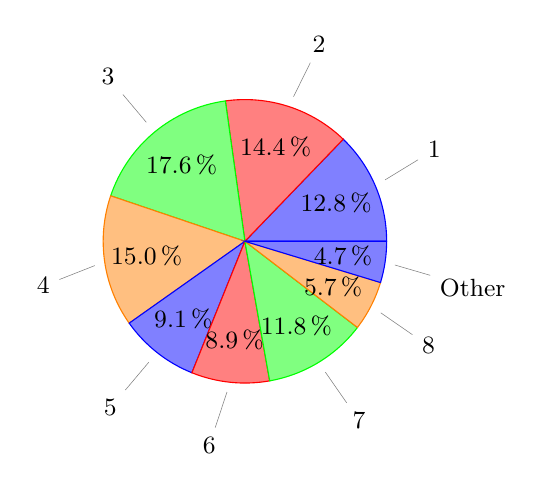
\begin{tikzpicture}[nodes = {font=\small},scale=.6]
  		\foreach \percent/\name in {
      		12.8/1,
      		14.4/2,
      		17.6/3,
      		15.0/4,
      		9.1/5,
      		8.9/6,
      		11.8/7,
      		5.7/8,
      		4.7/Other       
    	} {
      	\ifx\percent\empty\else               % If \percent is empty, do nothing
        \global\advance\cyclecount by 1     % Advance cyclecount
        \global\advance\ind by 1            % Advance list index
        \ifnum3<\cyclecount                 % If cyclecount is larger than list
        \global\cyclecount=0              %   reset cyclecount and
        \global\ind=0                     %   reset list index
        \fi
        \pgfmathparse{\cyclelist[\the\ind]} % Get color from cycle list
        \edef\color{\pgfmathresult}         %   and store as \color
        % Draw angle and set labels
        \draw[fill={\color!50},draw={\color}] (0,0) -- (\angle:\radius)
          	arc (\angle:\angle+\percent*3.6:\radius) -- cycle;
        \node at (\angle+0.5*\percent*3.6:0.7*\radius) {\percent\,\%};
        \node[pin=\angle+0.5*\percent*3.6:\name]
          	at (\angle+0.5*\percent*3.6:\radius) {};
        \pgfmathparse{\angle+\percent*3.6}  % Advance angle
        \xdef\angle{\pgfmathresult}         %   and store in \angle
      	\fi
    };
	\end{tikzpicture}
	}

	\caption{Years Spent at Job}
	\label{fig:node pie job}
\end{subfigure}

\hspace*{-7cm}\begin{subfigure}[h]{.25\linewidth}

	% Pie chart with colors
	% Author: Henri Menke
	\def\angle{0}
	\def\radius{3}
	\def\cyclelist{{"orange","blue","red","green"}}
	\newcount\cyclecount \cyclecount=-1
	\newcount\ind \ind=-1
	\resizebox {98mm} {!} {
	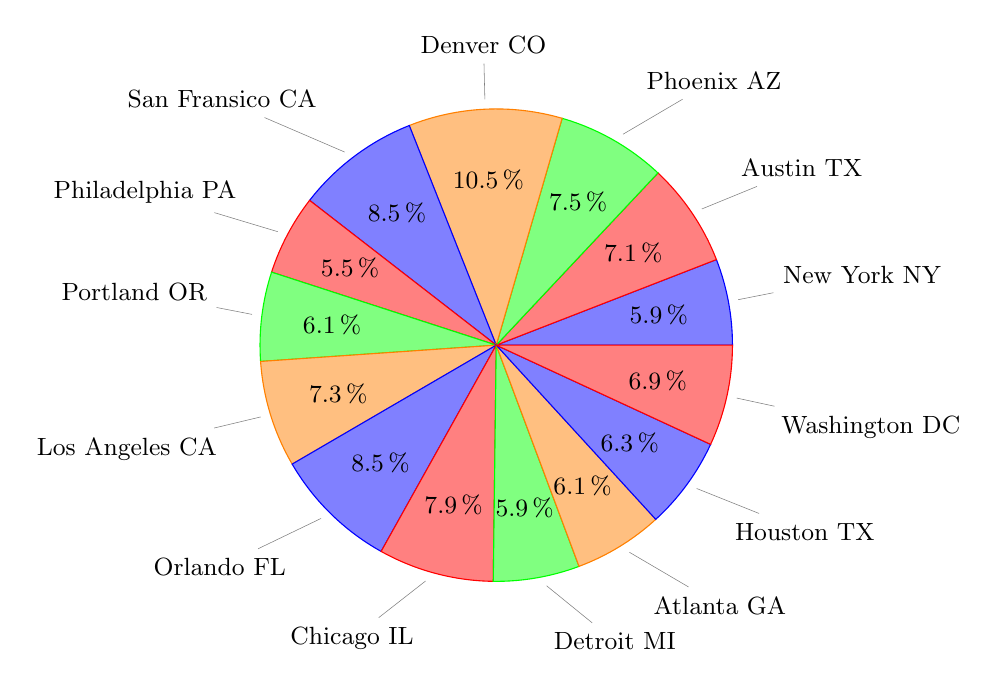
\begin{tikzpicture}[nodes = {font=\small}]
  		\foreach \percent/\name in {
			5.9/New York NY,
			7.1/Austin TX,
			7.5/Phoenix AZ,
			10.5/Denver CO,
			8.5/San Fransico CA,
			5.5/Philadelphia PA,
			6.1/Portland OR,
			7.3/Los Angeles CA,
			8.5/Orlando FL,
			7.9/Chicago IL,
			5.9/Detroit MI,
			6.1/Atlanta GA,
			6.3/Houston TX,
			6.9/Washington DC      
    	} {
      	\ifx\percent\empty\else               % If \percent is empty, do nothing
        \global\advance\cyclecount by 1     % Advance cyclecount
        \global\advance\ind by 1            % Advance list index
        \ifnum3<\cyclecount                 % If cyclecount is larger than list
        \global\cyclecount=0              %   reset cyclecount and
        \global\ind=0                     %   reset list index
        \fi
        \pgfmathparse{\cyclelist[\the\ind]} % Get color from cycle list
        \edef\color{\pgfmathresult}         %   and store as \color
        % Draw angle and set labels
        \draw[fill={\color!50},draw={\color}] (0,0) -- (\angle:\radius)
          	arc (\angle:\angle+\percent*3.6:\radius) -- cycle;
        \node at (\angle+0.5*\percent*3.6:0.7*\radius) {\percent\,\%};
        \node[pin=\angle+0.5*\percent*3.6:\name]
          	at (\angle+0.5*\percent*3.6:\radius) {};
        \pgfmathparse{\angle+\percent*3.6}  % Advance angle
        \xdef\angle{\pgfmathresult}         %   and store in \angle
      	\fi
    	};
	\end{tikzpicture}
	}
	
	\caption{Job Location}
	\label{fig:node pie job}
\end{subfigure}

\caption{Lead Architect}
\label{fig:Lead Arch}
\end{figure}

To demonstrate the ease at which the data can be generated and shown through
this tool, several modifications are now made to this example.  First, a second
degree is added to Civil Engineer but it is only 33\% likely to occur between
the two.  This is done by adding the following line to the Masters text file.

	\indent \textit{Civil:Infrastructure,Energy,Infrastructure}\\*

\noindent Next, an additional node, Junior Partner is added prior to Partner. 
This is done by modify the Titles text file.  To make this change, the simple
replacement of one line with two new lines was needed.
	
	\indent Remove}\textit{Lead Architect:Partner}\\*
	\indent Add:\textit{Lead Architect:Junior Partner}\\*
	\indent Add:\textit{Junior Partner:Partner}\\*
	
\noindent Finally, the likelihood of someone obtaining a Master's degree was
reduced by incrementing the m\_chance variable by 2 in the User Data Generation
Perl script.



\usetikzlibrary{shapes,arrows,chains}

\begin{figure}[H]
	\centering
  
% Start the picture
\resizebox {150mm} {!} {
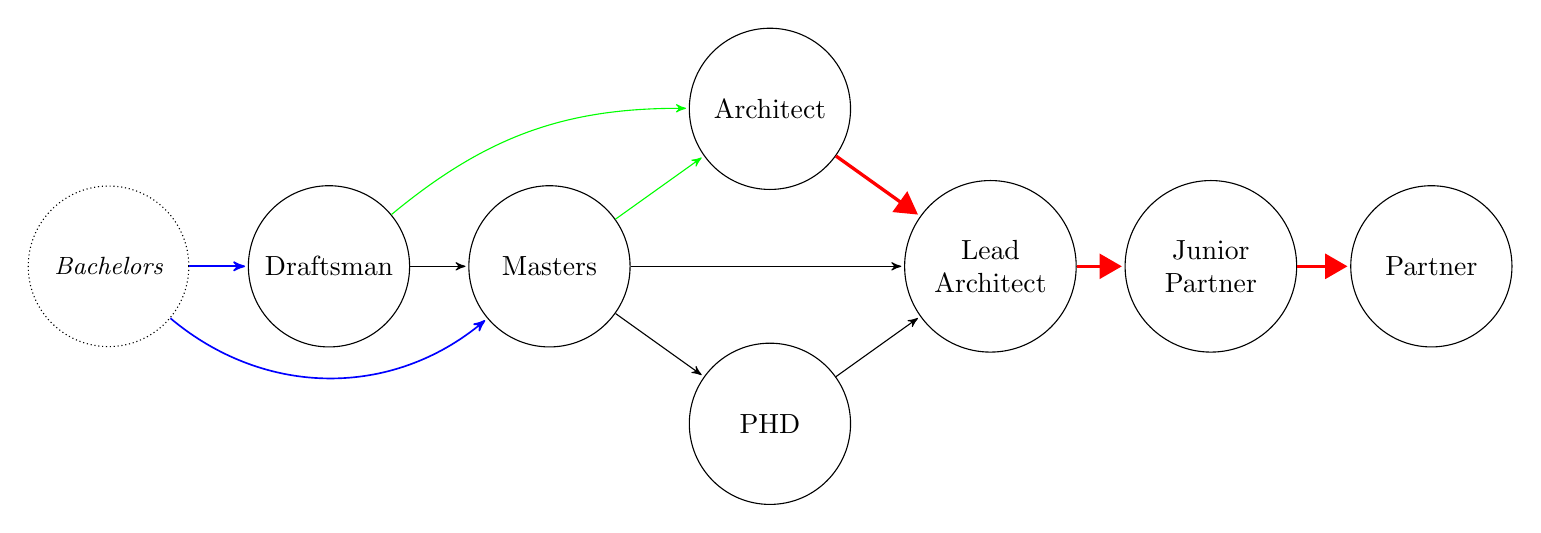
\begin{tikzpicture}[%
    >=triangle 60,              % Nice arrows; your taste may be different
    start chain=going below,    % General flow is top-to-bottom
    node distance=3mm and 28mm, % Global setup of box spacing
    every join/.style={norm},   % Default linetype for connecting boxes
    ]
% ------------------------------------------------- 
% A few box styles 
% <on chain> *and* <on grid> reduce the need for manual relative
% positioning of nodes

\tikzset{
  base/.style={draw, on chain, on grid, align=center, minimum height=2ex},
  node/.style={base, circle, text width=5em},
  % Connector line styles for different parts of the diagram
  norm/.style={->, draw},
  thin/.style={->,>=stealth',shorten >=1pt, black},
  nm/.style={->,>=stealth',shorten >=1pt, green},
  to/.style={->,>=stealth',shorten >=1pt,semithick,blue},
  thick/.style={->,shorten >=1pt,very thick, red},
  it/.style={font={\small\itshape}}
}
% -------------------------------------------------
% Start by placing the nodes
\node [node, densely dotted, it] (a) {Bachelors};
% Use join to connect a node to the previous one 
\node [node, right = of a] (b) {Draftsman};
\node [node, right = of b] (c) {Masters}; 
\node [node, right = of c, yshift=20mm] (d) {Architect};
\node [node, right = of c, yshift=-20mm] (e) {PHD};
\node [node, right = of e, yshift=20mm] (f) {Lead Architect};
\node [node, right = of f] (g) {Junior Partner};
\node [node, right = of g] (h) {Partner};

\draw[to] (a) to (b);		%Bachelors,Draftsman,5
\draw[nm] (b) to [bend left=20] (d);		%Draftsman,Architect,4
\draw[thick] (d) to (f);		%Architect,Lead Architect,7
\draw[thick] (f) to (g);	%Lead Architect,Junior Partner,10
\draw[thick] (g) to (h);	%Junior Partner,Partner,10
\draw[to] (a) to [bend right=40] (c);		%Bachelors,Masters,4
\draw[nm] (c) to (d); 	%Masters,Architect,2
\draw[thin] (c) to (f);		%Masters,Lead Architect,1
\draw[thin] (c) to (e);		%Masters,PHD,0
\draw[thin] (e) to (f);		%PHD,Lead Architect,0
\draw[thin] (b) to (c);		%Draftsman,Masters,0

% -------------------------------------------------
\end{tikzpicture}
}

	\caption{Modified Career Path Nodal Map}
	\label{fig:mod partner nodal map}
\end{figure}

With the changes in place, the new career map for achieving the Partner
position shows the new node step of Junior Partner.  It also shows the reduction
of users obtain a Master's degree.  In the case of users transitioning from a
Bachelor's to Master's degree, it is not clear from the colors, but looking at
the actual return data, the frequency did decrease by 10\%.  Upon gathering the
data for the Master's Degree node, it also shows that Infrastructure degrees now
make up approximately 2/3rds of the degrees.  This is shown in the JSON
return for the Masters node with the following text:

\indent Data Breakout"\\*
\indent \indent \indent \{"name":"Infrastructure","value":"61.50794\%"\},\\*
\indent \indent \indent \{"name":"Energy","value":"38.49206\%"\}

\noindent Additionally, both Infrastructure and Energy would be returned as
significant pieces of data as they occur much more frequently than all of the
users who traveled through this Master's degree node.

\subsection{Example Carrer Map }
Consider another user who is interested in reaching the System Chief Engineering
role.  They would input this query into the tool and figure \ref{fig:node map
sce} would be generated.  From this map, the user would quickly be able to see
that obtaining an advanced degree was unnecessary to become a System Chief
Engineer.  They could then delve deeper into each node if they wanted to learn
more about users who did the various jobs that also became System Chief
Engineers.


\usetikzlibrary{shapes,arrows,chains}

\begin{figure}[H]
	\centering
  
% Start the picture
\resizebox {150mm} {!} {
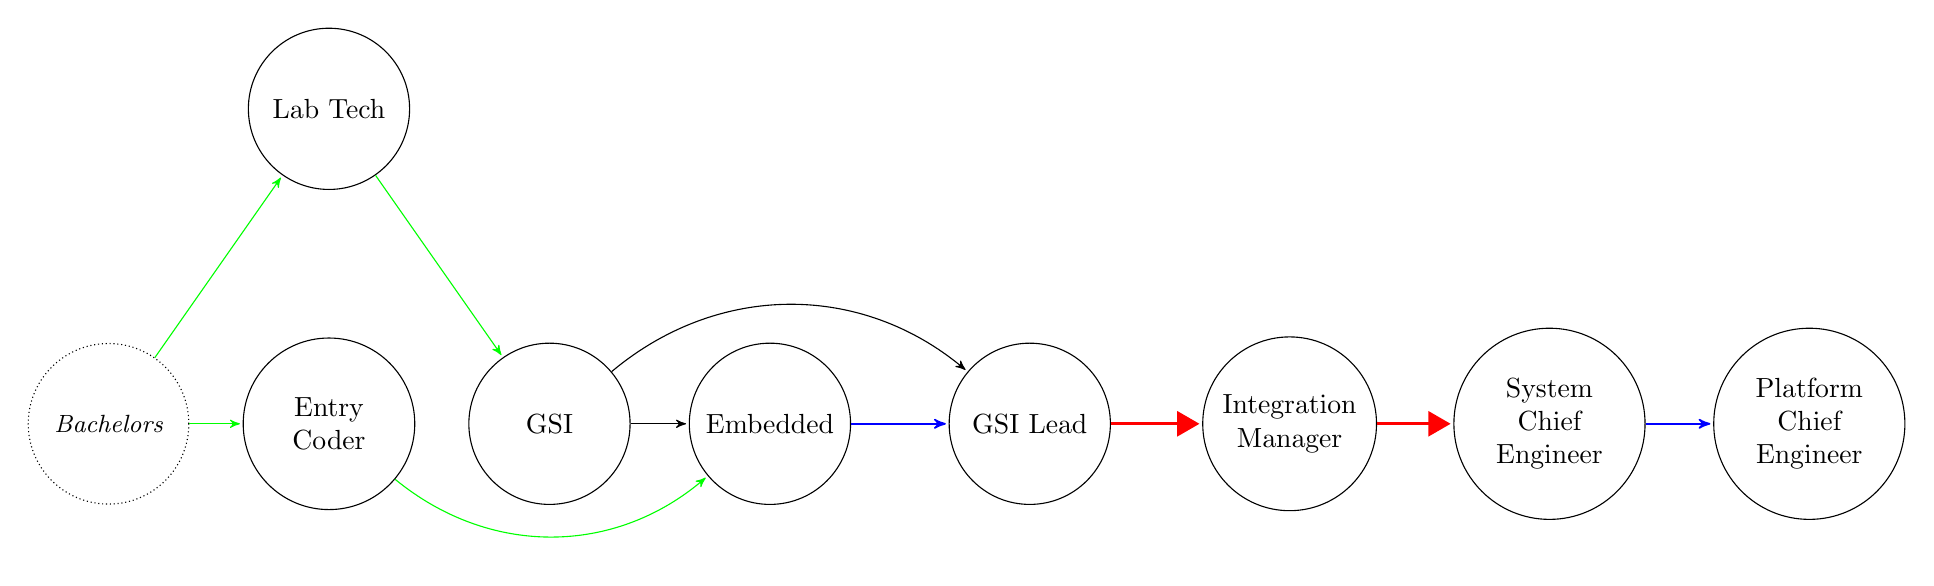
\begin{tikzpicture}[%
    >=triangle 60,              % Nice arrows; your taste may be different
    start chain=going below,    % General flow is top-to-bottom
    node distance=3mm and 28mm, % Global setup of box spacing
    every join/.style={norm},   % Default linetype for connecting boxes
    ]
% ------------------------------------------------- 
% A few box styles 
% <on chain> *and* <on grid> reduce the need for manual relative
% positioning of nodes
\tikzset{
  base/.style={draw, on chain, on grid, align=center, minimum height=2ex},
  node/.style={base, circle, text width=5em},
  % Connector line styles for different parts of the diagram
  norm/.style={->, draw},
  thin/.style={->,>=stealth',shorten >=1pt, black},
  nm/.style={->,>=stealth',shorten >=1pt, green},
  to/.style={->,>=stealth',shorten >=1pt,semithick,blue},
  thick/.style={->,shorten >=1pt,very thick, red},
  it/.style={font={\small\itshape}}
}
% -------------------------------------------------
% Start by placing the nodes

\node [node, densely dotted, it] (a) {Bachelors};
% Use join to connect a node to the previous one 
\node [node, right = of a,yshift=0mm] (b) {Entry Coder};
\node [node, right = of a,yshift=40mm] (c) {Lab Tech}; 
\node [node, right = of b] (d) {GSI};
\node [node, right = of d] (e) {Embedded};
\node [node, right = of e,xshift=5mm] (f) {GSI Lead};
\node [node, right = of f,xshift=5mm] (g) {Integration Manager};
\node [node, right = of g,xshift=5mm] (h) {System Chief Engineer};
\node [node, right = of h,xshift=5mm] (i) {Platform Chief Engineer}; 

\draw[nm] (a) to (c);		%Bachelors,Lab Tech,7
\draw[nm] (c) to (d);		%Lab Tech,GSI,7
\draw[thin] (d) to [bend left=40] (f);		%GSI,GSI Lead,4
\draw[thick] (f) to (g);		%GSI Lead,Integration Manager,14
\draw[thick] (g) to (h);		%Integration Manager,System Chief Engineer,14
\draw[to] (h) to (i);		%System Chief Engineer,Platform Chief Engineer,11
\draw[nm] (a) to (b);		%Bachelors,Entry Coder,7
\draw[nm] (b) to [bend right=40] (e);		%Entry Coder,Embedded,7
\draw[to] (e) to (f);		%Embedded,GSI Lead,10
\draw[thin] (d) to (e);		%GSI,Embedded,3

% -------------------------------------------------
\end{tikzpicture}
}

	\caption{System Chief Engineer Nodal Map}
	\label{fig:node map sce}
\end{figure}

One thing that might also spark an interest in the user is the fact that any
jobs beyond the queried job that the matched users also completed would be shown
as well.  In this case there was one of these such nodes, the Platform Chief
Engineer.  From the node transitions it is clear that not all System Chief
Engineers reached this job.  If the user were interested then instead in the
Platform Chief Engineering role, they could re-run the query and they would be
presented with the career map shown in figure \ref{fig:node map pce}.  This is
obviously a much more complex map, but it still yields the same capability of
quickly showing users complex career paths to a particular goal.  In this case
it shows that there are essentially three paths to this job.  The first path was
detailed in the initial query, the second path is through a Design career
path, and the third path is through an advanced degree.  What is most notable
about these paths is if the advanced degree path is taken, the initial jobs
the users take don't have much impact, as long as it is within the career realm.
The other notable thing is the most common path taken to getting to the Platform
Chief Engineering job is through the design path.


\usetikzlibrary{shapes,arrows,chains}

\begin{figure}[H]
	\centering
  
% Start the picture
\resizebox {!} {190mm} {
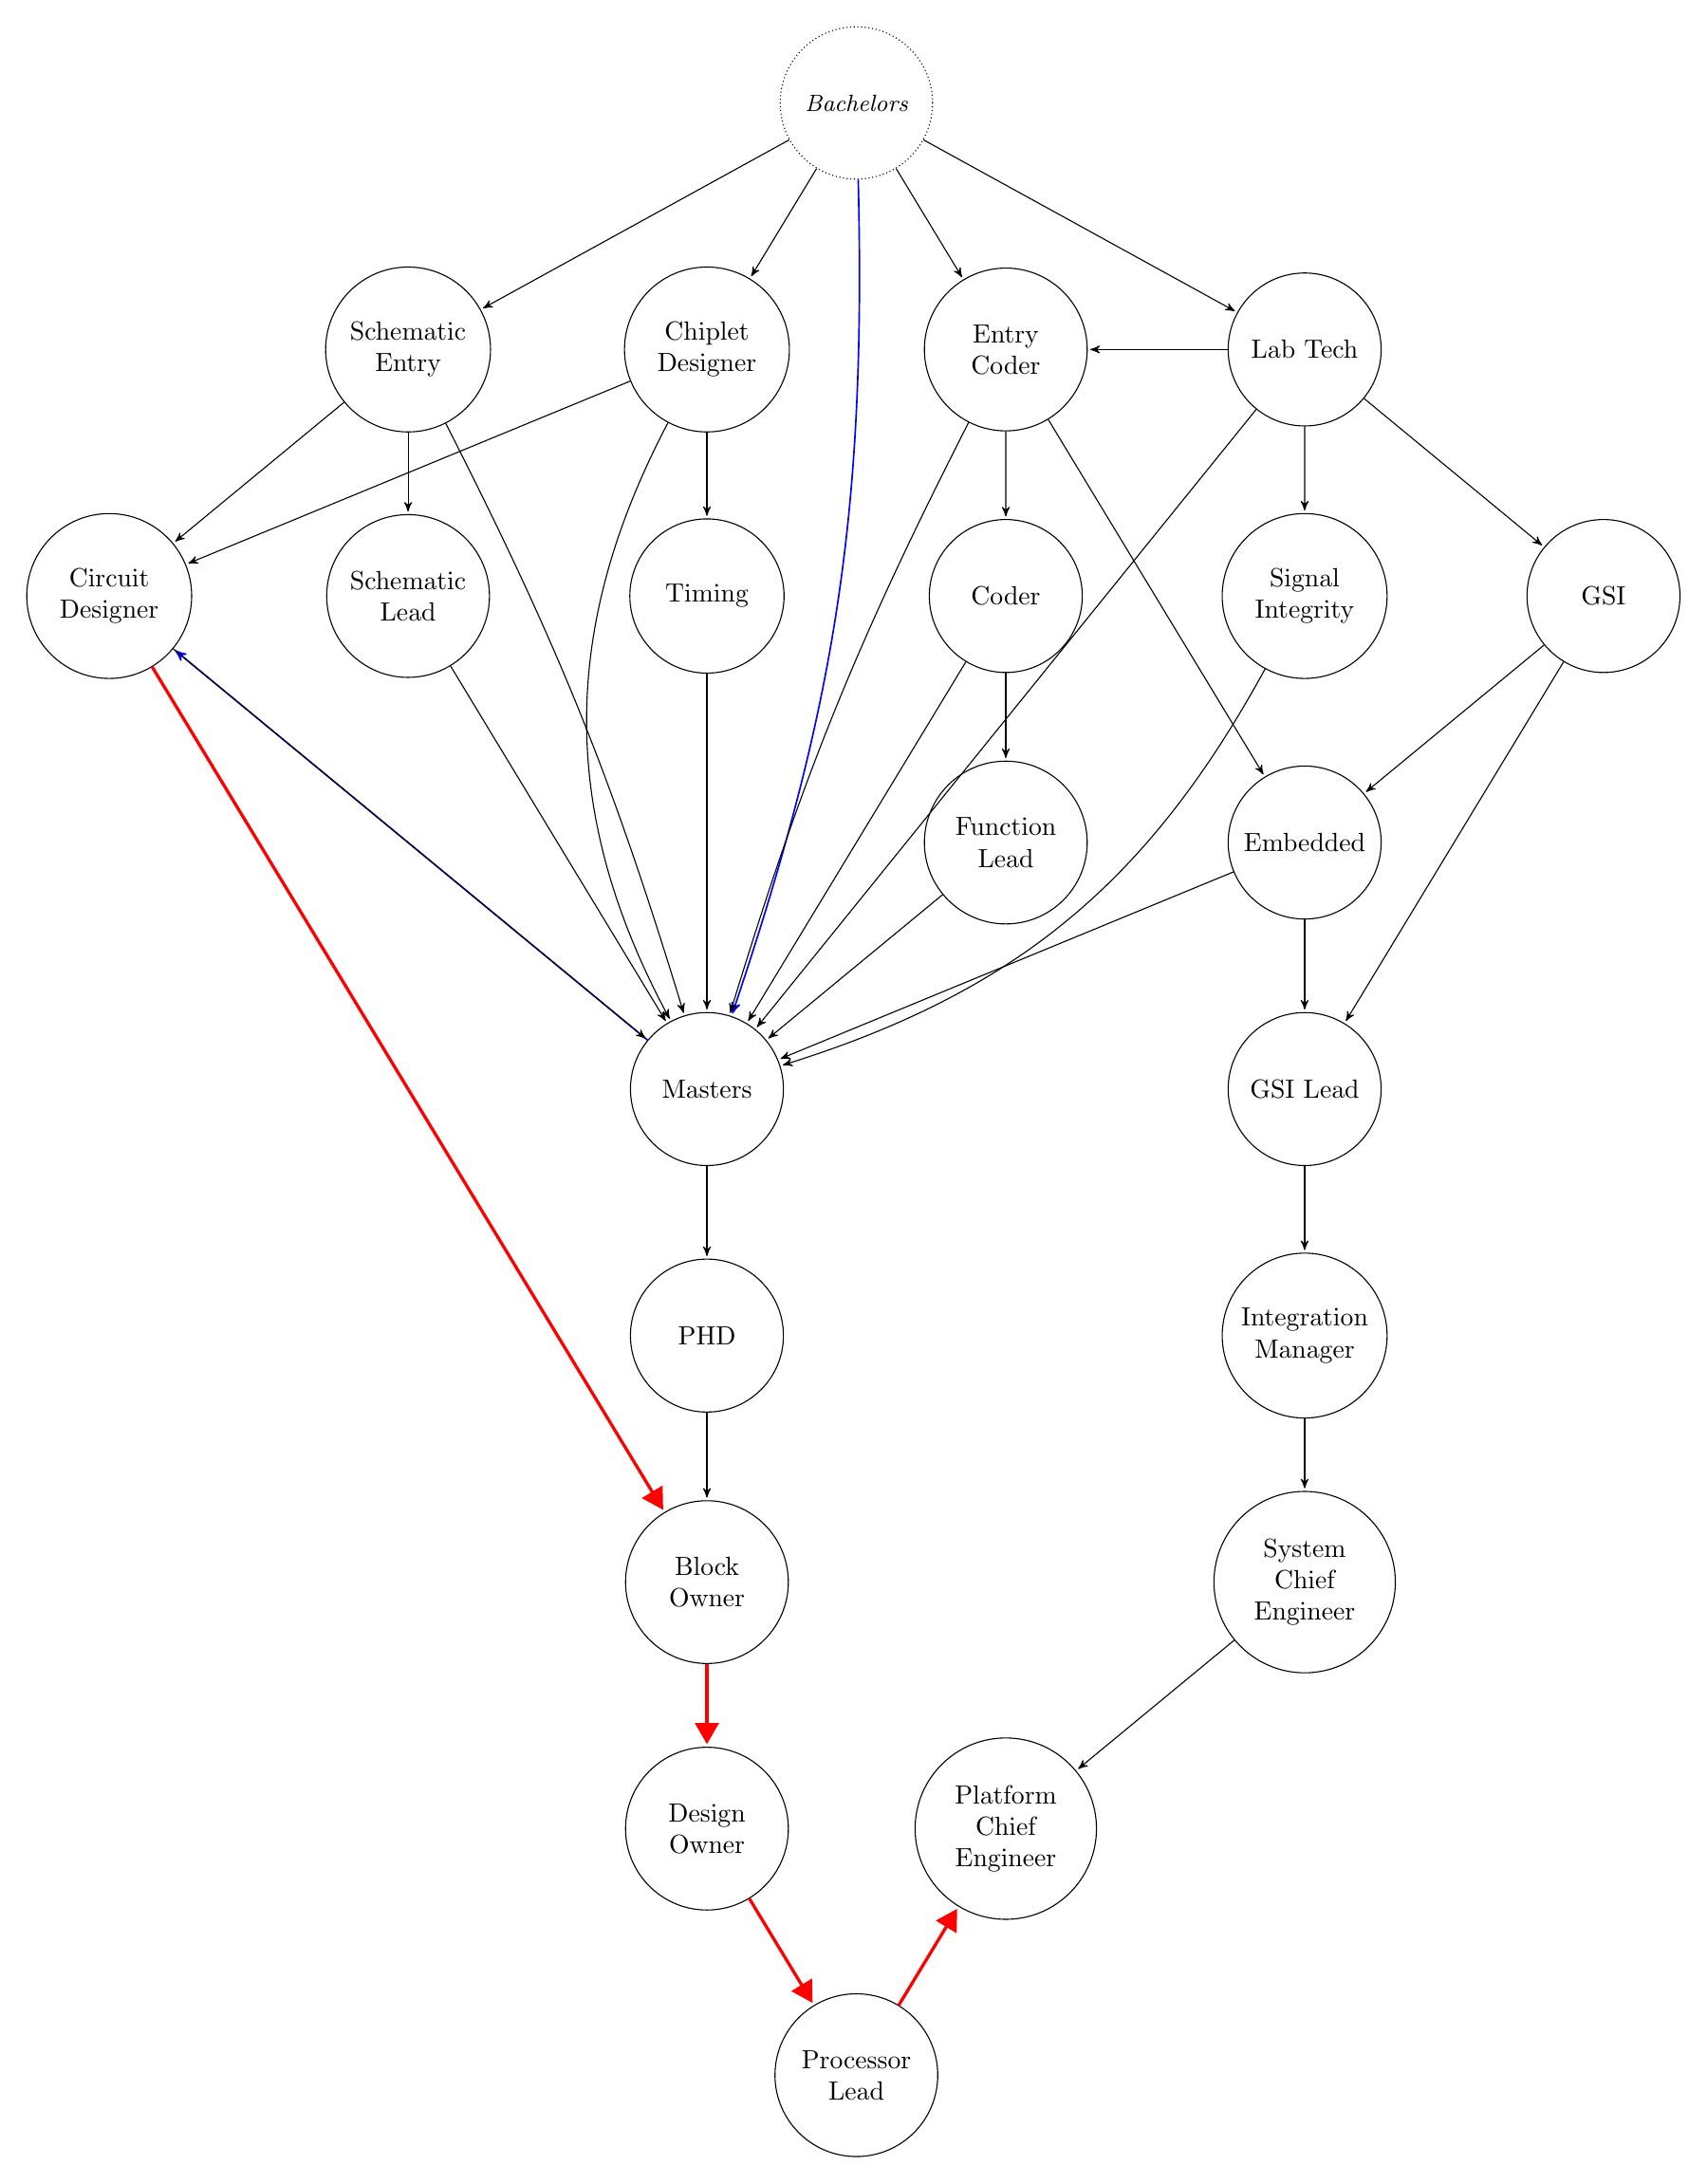
\begin{tikzpicture}[%
    >=triangle 60,              % Nice arrows; your taste may be different
    start chain=going below,    % General flow is top-to-bottom
    node distance=3mm and 28mm, % Global setup of box spacing
    every join/.style={norm},   % Default linetype for connecting boxes
    ]
% ------------------------------------------------- 
% A few box styles 
% <on chain> *and* <on grid> reduce the need for manual relative
% positioning of nodes
\tikzset{
  base/.style={draw, on chain, on grid, align=center, minimum height=2ex},
  node/.style={base, circle, text width=5em},
  % Connector line styles for different parts of the diagram
  norm/.style={->, draw},
  thin/.style={->,>=stealth',shorten >=1pt, black},
  nm/.style={->,>=stealth',shorten >=1pt, green},
  to/.style={->,>=stealth',shorten >=1pt,semithick,blue},
  thick/.style={->,shorten >=1pt,very thick, red},
  it/.style={font={\small\itshape}}
}
% -------------------------------------------------
% Start by placing the nodes

\node [node, densely dotted, it] (a) {Bachelors};
% Use join to connect a node to the previous one 
\node [node, below = of a,yshift=-30mm,xshift=20mm] (b) {Entry Coder};
\node [node, below = of a,yshift=-30mm,xshift=60mm] (c) {Lab Tech}; 
\node [node, below = of a,yshift=-30mm,xshift=-60mm] (d) {Schematic Entry};
\node [node, below = of a,yshift=-30mm,xshift=-20mm] (e) {Chiplet Designer};
\node [node, below = of d,yshift=-30mm,xshift=40mm] (f) {Timing};
\node [node, below = of d,yshift=-30mm,xshift=120mm] (g) {Signal Integrity};
\node [node, below = of d,yshift=-30mm,xshift=-40mm] (h) {Circuit Designer};
\node [node, below = of d,yshift=-30mm,xshift=80mm] (i) {Coder};
\node [node, below = of d,yshift=-30mm,xshift=0mm] (j) {Schematic Lead};
\node [node, below = of d,yshift=-30mm,xshift=160mm] (k) {GSI};
\node [node, below = of i,yshift=-30mm] (l) {Function Lead};
\node [node, below = of i,yshift=-30mm,xshift=40mm] (m) {Embedded};
\node [node, below = of l,yshift=-30mm,xshift=-40mm] (n) {Masters};
\node [node, below = of l,yshift=-30mm,xshift=40mm] (o) {GSI Lead};
\node [node, below = of n,yshift=-30mm] (p) {PHD};
\node [node, below = of o,yshift=-30mm] (q) {Integration Manager};
\node [node, below = of q,yshift=-30mm] (r) {System Chief Engineer};
\node [node, below = of p,yshift=-30mm] (s) {Block Owner};
\node [node, below = of s,yshift=-30mm,xshift=40mm] (t) {Platform Chief
Engineer}; 
\node [node, below = of s,yshift=-30mm] (u) {Design Owner};
\node [node, below = of u,yshift=-30mm,xshift=20mm] (v) {Processor Lead};

\draw[to] (a) to [bend left=10] (n);		%Bachelors,Masters,6
\draw[to] (n) to (h);		%Masters,Circuit Designer,7
\draw[thick] (h) to (s);		%Circuit Designer,Block Owner,8
\draw[thick] (s) to (u);		%Block Owner,Design Owner,9
\draw[thick] (u) to (v);		%Design Owner,Processor Lead,9
\draw[thick] (v) to (t);		%Processor Lead,Platform Chief Engineer,9
\draw[thin] (a) to (d);		%Bachelors,Schematic Entry,0
\draw[thin] (d) to (j);		%Schematic Entry,Schematic Lead,0
\draw[thin] (j) to (n);		%Schematic Lead,Masters,0
\draw[thin] (n) to (p);		%Masters,PHD,1
\draw[thin] (p) to (s);		%PHD,Block Owner,1
\draw[thin] (d) to [bend left=5](n);		%Schematic Entry,Masters,0
\draw[thin] (a) to (c);		%Bachelors,Lab Tech,1
\draw[thin] (c) to (k);		%Lab Tech,GSI,0
\draw[thin] (k) to (o);		%GSI,GSI Lead,0
\draw[thin] (o) to (q);		%GSI Lead,Integration Manager,1
\draw[thin] (q) to (r);		%Integration Manager,System Chief Engineer,1
\draw[thin] (r) to (t);		%System Chief Engineer,Platform Chief Engineer,1
\draw[thin] (a) to (b);		%Bachelors,Entry Coder,1
\draw[thin] (b) to (i);		%Entry Coder,Coder,0
\draw[thin] (i) to (n);		%Coder,Masters,0
\draw[thin] (c) to (b);		%Lab Tech,Power,0
\draw[thin] (b) to (m);		%Entry Coder,Embedded,0
\draw[thin] (m) to (n);		%Embedded,Masters,0
\draw[thin] (c) to (n);		%Lab Tech,Masters,0
\draw[thin] (b) to [bend right=5] (n);		%Entry Coder,Masters,0
\draw[thin] (m) to (o);		%Embedded,GSI Lead,0
\draw[thin] (d) to (h);		%Schematic Entry,Circuit Designer,0
\draw[thin] (a) to (e);		%Bachelors,Chiplet Designer,0
\draw[thin] (e) to [bend right=28] (n);		%Chiplet Designer,Masters,0
\draw[thin] (k) to (m);		%GSI,Embedded,0
\draw[thin] (e) to (h);		%Chiplet Designer,Circuit Designer,0
\draw[thin] (c) to (g);		%Lab Tech,Signal Integrity,0
\draw[thin] (g) to [bend left=22](n);		%Signal Integrity,Masters,0
\draw[thin] (e) to (f);		%Chiplet Designer,Timing,0
\draw[thin] (f) to (n);		%Timing,Masters,0
\draw[thin] (h) to (n);		%Circuit Designer,Masters,0
\draw[thin] (i) to (l);		%Coder,Function Lead,0
\draw[thin] (l) to (n);		%Function Lead,Masters,0

% -------------------------------------------------
\end{tikzpicture}
}

	\caption{Platform Chief Engineer Nodal Map}
	\label{fig:node map pce}
\end{figure}


\subsection{Career Path Performance}
All of the work on this project has been done on a personal laptop with an 8
core i7 2.70GHz processor, a 500GB 7200 RPM 32MB Cache SATA 6.0Gb/s hard drive,
and 16GB of DDR3 Memory.  As ProGENitor would be run on a server instead of a
personal laptop, it can be expected that the performance for all workloads would
be improved.  Still, the overall application run time would be impacted by both
the number of users within the database and the total access times to the
database itself.  As the database was on a local drive, the access times were
much less in these run times than they could be with a remote database.  

For generating the career path map, 10 cases were run, as shown below in table
\ref{table:career performance}.  These 10 cases generate a range of matched
users, total users, and number of nodes returned.  By doing this, a ruff estimate as to how
long a query to ProGENitor might take can be ascertained.  As seen in table
\ref{table:career performance}, an average query would take about 2.5 seconds,
but might take much longer depending on the number of users in the database and the number that
match the query.  One thing to note about the data in these tables is that there
is currently a bug in the ProGENitor code that forced a cap of 500 matched
users.  Any number of matched users returned beyond that 500 is currently
ignored.  This does not invalidate the data and may be something that is deisred
simply to improve overall performance.  In the future this issue would be
resolved, but for now, please note this limiting factor when looking over the
data in the following tables.

\begin{table}[H]
  \centering
  \begin{tabular}{|p{17mm}|p{16mm}|p{10mm}|p{18mm}|p{19mm}|p{20mm}|p{14mm}|}
  \hline
  \
  %heading
  Case&Matched Users&Total Users&Data\newline Collection&Edge\newline
  Generation&Order Generation&Total\\
  \hline\hline
  Platform Chief&109&5000&708.9ms&341.4ms&74.4ms&1.12s\\ \hline
  Civil\newline Degree&2684&5000&2.28s&2.37s&6.3ms&4.65s\\ \hline 
  Architect&2330&5000&2.27s&2.19s&5.7ms&4.47s\\ \hline
  Circuit Designer&675&5000&2.23s&1.0s&68.5ms&3.3s\\ \hline
  Worked For IBM&260&5000&1.31s&457.5ms&85.6ms&1.85s\\ \hline
  Fission Degree&260&5000&1.31s&407.6ms&6.3ms&1.73s\\ \hline
  Analog Degree&24&5000&361.2ms&66.8ms&43.1ms&471.3ms\\ \hline
  Embedded&55&5000&466.8ms&269.5ms&94.7ms&831.1ms\\ \hline
  Floor- \newline planning&49&5000&441.5ms&106.5ms&103.3ms&651.5ms\\ \hline
  Circuit Designer&1401&10000&4.27s&1.72s&70.8ms&6.06s\\ \hline
  \hline\hline
  Minimum&24&5000&361.2ms&66.8ms&5.7ms&471.3ms\\ \hline
  Maximum&2684&10000&4.27s&2.37s&103.3ms&6.06s\\ \hline
  Average&785&550&1.55s&893ms&55.9ms&2.5s\\ \hline
  \end{tabular}
  \label{table:career performance}
  \caption{Career Path Generation Time}
\end{table}

As seen in table \ref{table:career performance}, the bulk of the time that
ProGENitor runs is spent in querying the database and pulling in the data to be
processed.  Then generating the node interconnects takes up about a third of the
run time. Lastly, determining the order in which to display the nodes runs in
about 1 to 2\% of the overall runtime.  Thus, to improve or maintain performance most of
the focus needs to be on the database pull.  This is not an uncommon problem and
many people spend careers working on this problem.  ProGENitor assumes that
whoever deploys the tool would either have a smaller database or a database
expert who could help refine the database accesses.

\begin{table}[H]
  \centering
  \begin{tabular}{|p{17mm}|p{16mm}|p{10mm}|p{18mm}|p{19mm}|p{20mm}|}
  \hline
  \
  %heading
  Case&Matched Users&Total Users&Total Nodes&All Nodes&Average Node\\
  \hline\hline
  Platform Chief&109&5000&23&4.7s&204.4ms\\ \hline
  Civil\newline Degree&2684&5000&7&6.34s&906.3ms\\ \hline 
  Architect&2330&5000&6&6.15s&1.02s\\ \hline
  Circuit Designer&675&5000&32&7.79s&243.5ms\\ \hline
  Worked For IBM&260&5000&40&6.8s&170.1ms\\ \hline
  Fission Degree&260&5000&6&1.72s&653.8ms\\ \hline
  Analog Degree&24&5000&12&3.94s&328.6ms\\ \hline
  Embedded&55&5000&30&5.1s&170.1ms\\ \hline
  Floor- \newline planning&49&5000&18&4.6s&155.2ms\\ \hline
  Circuit Designer&1401&10000&31&13.0s&419.7ms\\ \hline
  \hline\hline
  Minimum&24&5000&6&1.72s&155.2ms\\ \hline
  Maximum&2684&10000&40&13.0s&1.02s\\ \hline
  Average&785&550&20.5&6.0s&427.2ms\\ \hline
  \end{tabular}
  \label{table:node-perf}
  \caption{Node Detail Generation Time}
\end{table}

In table \ref{table:node-perf}, the node detail generation performance is shown
for the same 10 cases run previously.  This is broken out seperately because the
assumption is that when ProGENitor is deployed the career map would be initially
presented in the user interface and the details about each node would be
displayed upon user request.  Looking at table \ref{table:node-perf} shows that
this would be done because if all the data were returned at once, it could
potentially add 13 seconds to the overall run time.  This would be too slow and
unecessary for the end user.  By making each node call seperate, the average
return time on the node information would be about half a second prior to
rendering the data.  This would make the data much more user friendly.